%%%%%%%%%%%%%%%%%%%%%%%%%%%%%%%%%%%%%%%%%
% Friggeri Resume/CV
% XeLaTeX Template
% Version 1.2 (3/5/15)
%
% This template has been downloaded from:
% https://github.com/mlda065/friggeri-letter
%
% Original author:
% Adrien Friggeri (adrien@friggeri.net)
% https://github.com/afriggeri/CV
%
% Modifications by Luc Vanrobays (luc.vanrobays@gmail.com)
%
% License:
% CC BY-NC-SA 3.0 (http://creativecommons.org/licenses/by-nc-sa/3.0/)
%
% Important notes:
% This template needs to be compiled with XeLaTeX
%
%%%%%%%%%%%%%%%%%%%%%%%%%%%%%%%%%%%%%%%%%

\documentclass[a4paper]{myfriggeri-cv}
% Add 'print' as an option into the square bracket to remove colors from this template for printing
% Add `a4paper` to set a4 paper size
% Add `nocolors` to remove colors from the document
% Add `lightheader` to change the dark background of the header to white
\usepackage[brazil]{babel}
\usepackage{unicode-math}
\usepackage{csquotes}
\usepackage{fontawesome}
\usepackage{array} % otherwise you get "Error: Illegal character in array arg."
\usepackage{booktabs}			% Better tables
\usepackage{tabulary}			% Support longer table cells
\definecolor{light-gray}{gray}{0.55}
\definecolor{skype}{HTML}{12A5F4}
\definecolor{html5}{HTML}{e34c26}
\definecolor{php}{HTML}{6c7eb7}
\definecolor{db}{HTML}{FF9900}
\definecolor{linkedin}{HTML}{1683BB}
%\addbibresource{bibliography.bib} % Specify the bibliography file to include publications

\begin{document}
\newfontfamily{\FA}{FontAwesome}
\providecommand\faSkype{{\FA\symbol{"F17E}}}
\header{Carlos}{Fulano}{Franchise Sales Manager} % Your name and current job title/field

%----------------------------------------------------------------------------------------
%	SIDEBAR SECTION
%----------------------------------------------------------------------------------------
\aside{contato}{
%don't display the name in the contact details on the first page
%because it's up the top
%That's why there's the if statement
\ifx \firstPage \undefined
   \xdef\firstPage{}
\else
Carlos Fulano \\
~ \\
\fi
São Paulo \\
Brasil \\
~  \\
+55 (11) 89562-5324 \\
~   \\
\href{mailto: carlos@hotmail.com}{ carlos@hotmail.com} \\
%\section{\includegraphics[scale=0.05]{linkedinLogo.png}} %or
\section{\linkedInLogoTikz{0.4}}{\href{http://linkedin.com/in/carlos-fulano}{carlos-fulano}}\\
\faSkype{carlosodeplancton}
~   \\
~   \\
%uncomment for picture on each page
%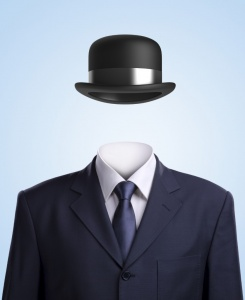
\includegraphics[width=0.325\textwidth]{Jagan_round.jpg}
%%\section{\skypeLogoTikz{0.4}}
%{skype:lucodealethea?call}
}
\section{}
{Carlos tem grande experiência,\emph{equilibrando} processos de negócio na vendas e em re-arquitetura de amplos sistemas (Utilities e Produtos de Consumo).
}
%--------------------------------------------------------------------------------
% EXPERIENCE SECTION
%--------------------------------------------------------------------------------
\section{Experiência}
\subsection{Projetos Pessoais}
\begin{entrylist}
\entry
{abr2013-presente}
{Privado}
{Pomerania,Tasmania,Fernando de Noronha}%side thing
{Dog Groomer}
{
Eu pratico dog grooming em \textbf{\MYhref[light-gray]{https://en.wikipedia.org/wiki/Open-source_model}{Código Aberto}}.
%------------------------------------------------
\begin{itemize}
\item{} O presente currículo foi escrito usando a linguagem \textbf{\MYhref[light-gray]{http://fletcherpenney.net/multimarkdown/}{MultiMarkDown}\slash \MYhref[light-gray]{https://www.latex-project.org/}{\LaTeX}}.
\item{}
Praticando Design Thinking.
\item{} Groomer \slash  Passeador cachorros (Evangelisto): 2013-2016
\end{itemize}
}
\end{entrylist}
%------------------------------------------------
\subsection{Treinamentos Recentes}
\begin{entrylist}
\entry
{}
{}
{}%side thing
{Treinamentos \textbf{\MYhref[light-gray]{http://www.lynda.com}{MOOC Lynda}} ou \textbf{\MYhref[light-gray]{http://www.udemy.com}{Udemy}} com certificados.}
{ \begin{itemize}
\item{} 2015:	Learning Squarespace
\item{} 2014:	Next Generation CSS Design with PostCSS and CSS
\end{itemize}
}
\end{entrylist}


\subsection{Experiência profissional}
\begin{entrylist}
%------------------------------------------------start subsection experienca1

\entry
{nov2012--mar2013}
{Magazine Roberta Ltda, BR}
{São Paulo,BR}%side thing
{Torcedor de Cabide}
{Para o \emph{\href{http://www.magazineluiza.com.br/}{Magazine}:}
\begin{itemize}
\item{}Realização e Prova de conceito de um aplicativo \textit{Venda de Cabide} para controle de \textit{roupas} e re–negociação.\\
\item{}Optimização de treinamentos em segurança incendios(de 300 reduzido a 80 minutos).
\end{itemize}
}
%------------------------------------------------

\entry
{set2012--nov2012}
{}
{São Paulo,BR}
{Vendedor-Camelot}
{Para \emph{\href{http://www.ldcom.com/br/pr/}{Louis Dreyfus Commodities}:}
\begin{itemize}
\item{}Venda esforçada de sacola de soja e outros comodidades a preço fora de serie.\\
\item{}Desenhar um conjunto de Regras de Descontos\slash Agregaçao multi-criteria para exportadoras.
\end{itemize}
}
%------------------------------------------------
\entry
{abr2011--mar2012}
{Grupo Groove Torantim Ltda}
{Rio de Janeiro,BR}%side thing
{Diretor de Vendas}
{Para \emph{\href{http://https://www.sagestart.com.br/}{Sage Brasileiro S.A}:}
\begin{itemize}
\item{} Responsavel da dinamização dos times de vendas e transmissão de relatórios tributários (SPED)eletrônicos de alta complexidade:
\end{itemize}
\begin{enumerate}
\item{} garantindo consistência entre varias Declarações Tributarias,Relatórios Financeiros e notas fiscais individuais(NFe)
\item{} para pagar contas tributarias e minimizar multas e juros proibitivos
\end{enumerate}
}
%------------------------------------------------end 3
%------------------------------------------------end subsection experienca1
\end{entrylist}
\subsection{}
\begin{entrylist}
%------------------------end 14-
\end{entrylist}
%------------------------------------------------end 11 subsection shadow 4
%	EDUCATION SECTION
%--------------------------------------------------------------------------------
\section{educação}
\begin{entrylist}
%------------------------------------------------
\entry
{1990--1995}
{Mestrado {\normalfont em Ciências Tributárias}}
{Universidade Católica de Buenos Aires,AR}
{Macroeconomia e Ciências Sociais}
{Marca Media Ponderada 78.1\%}
%------------------------------------------------
\entry
{2006--2011}
{Pós-graduação}
{Escola Estadual de Belem,CE}
{Ciências Agropecuarias,Comerciais e Industriais}
{
}
%------------------------------------------------
\end{entrylist}
%----------------------------------------------------------------------------------------
%	AWARDS SECTION
%----------------------------------------------------------------------------------------
\section{premiação}
\begin{entrylist}

%------------------------------------------------
\entry
{1999}
{Syngenta Award }
{Universidade Federal de Campina Grande, PB}
{Melhor Programação Arduino}
{}
%------------------------------------------------
\end{entrylist}
%----------------------------------------------------------------------------------------
%	Technical SKILLS SECTION
%----------------------------------------------------------------------------------------
\section{expertise técnica}
\begin{entrylist}
%------------------------------------------------
\entry
{}
{Software}
{}
{}
{
\begin{itemize}
\item{} Totus
\item{} Sage
\item{} SpedoFaz
\end{itemize}
}
%------------------------------------------------
\entry
{}
{Programação}
{}
{}
{
Efficiente com:
\begin{itemize}
\item{} JAVA EE 8
\item{} Ruby On Rails
\item{} Haskell
\end{itemize}
Confiante com:
\begin{itemize}
\item{} Visual Basic
\item{} PL/SQL
\item{} Adobe Acrobat
\item{} \LaTeX,Node.js
\item{} Vimtutor,Shell Script
\end{itemize}
}
%----------------------------------------------------
\entry
{}
{Metodologia - Frameworks - Otros - Sistemas Operativos}
{}
{}
{
\begin{itemize}
\item{} Merise: \textbf{\MYhref[light-gray]{https://en.wikipedia.org/wiki/Merise}{Merise}}
\item{} Metodologias:\textbf{\MYhref[light-gray]{https://en.wikipedia.org/wiki/General-purpose_modeling}{UML}}
\item{} CMS: Git,GitHub,GitKraken
\item{} Design Thinking: \textbf{\MYhref[light-gray]{https://www.build.me/splashapp/}{SAP Build}}
\item{} IDE: Eclipse Neon IDE,Brackets,MS Visual Studio
\item{} \textbf{\MYhref[light-gray]{http://www.baeyens.it/eclipse/}{Arduino IDE on Eclipse (Sloeber)}}
\end{itemize}
}
\end{entrylist}
%----------------------------------------------------------------------------------------
%	Languages SKILLS SECTION
%----------------------------------------------------------------------------------------
%\usepackage{booktabs}			% Better tables
%\usepackage{tabulary}			% Support longer table cells
\section{fluência em idiomas}
A1\slash A2,
B1\slash B2,
C1\slash C2.cfr.Rodapé:
\footnote{A1\slash A2: Utilizador básico,	B1\slash B2: Utilizador independente,C1\slash C2: Utilizador avançado de proficiência

\textbf{\MYhref[light-gray]{http://europass.cedefop.europa.eu/pt/resources/european-language-levels-cefr}{Níveis europeus – Grelha de auto-avaliação}}}
{
\begin{table}[htbp]
\begin{minipage}{\linewidth}
\setlength{\tymax}{0.6\linewidth}
\centering
\small
\begin{tabulary}{\textwidth}{@{}lccc@{}} \toprule
 \textbf{Idioma}   & \textbf{Entender   }& \textbf{Falar   }& \textbf{Escrever   }\\
\midrule

\textbf{Swahili}		 & C1		 & C1 	 & C1		 \\
\textbf{Norueguês}	 & C1		 & C1 	 & C1		 \\
\textbf{Francês}		 & C1		 & C1 	 & C1		 \\
\textbf{Espanhol}   & B1		 & B2 	 & B2		 \\
\textbf{Holandês}   & B1		 & B2 	 & B1		 \\
\bottomrule

\end{tabulary}
\end{minipage}
\end{table}
}
%------------------------------------------------
%----------------------------------------------------------------------------------------
%	Languages DIGITAL PROFICIENCY
%----------------------------------------------------------------------------------------
% In according to:
% europass.cedefop.europa.eu/resources/digital-competences
% The levels are:
%       Basic user			--> \ecvBasic
%       Independent user	--> \ecvIndependent
%       Proficient user		--> \ecvProficient
%
%  And the 5 areas of competence are:
%      Information processing
%      Content creation
%      Communication
%      Problem solving
%      Safety
%----------------------------------
\section{competência digital}

\section{certificados}
\begin{entrylist}
\entry
{}
{}
{}%side thing
{}
{ \begin{itemize}
\item{} 2012: OpenGoup – TOGAF Enterprise Architecture
\item{} 2011: Barry-Callebaut Chocolate Master Nr21247 (MCA)
\item{} 2004: Merchant Captain Master issued by Tobago Ministry of Maritime Affairs
\end{itemize}
}
\end{entrylist}
~
~
~
~

%------------------------------------------------
%----------------------------------------------------------------------------------------
%	Interests SECTION
%----------------------------------------------------------------------------------------
%\section{interesses}
%\begin{entrylist}
%------------------------------------------------
%\entry
%{}
%{}
%{}%side thing
%{}
%{ \begin{itemize}
%\item{} Literatura Nacional e Estrangeira
%\item{} Velejar,Esquiar,Correr,Trekking
%\item{} Cozinha Étnica,Antropologia e Geografia
%\item{} Artes,Cinema e Teatro
%\end{itemize}
%}
%\end{entrylist}
%----------------------------------------------------------------------------------------
%	Human SKILLS SECTION
%----------------------------------------------------------------------------------------
%\section{human skills}
%\begin{entrylist}
%------------------------------------------------
%\entry
%{}
%{Mentorship}
%{}
%{Carlos atuaou como Volumtario-Instrutor dee Voley por muitos anos,ensinando para muitos alunos e fãs
%}
%------------------------------------------------


%\entry
%{}
%{Teamwork}
%{}
%{}
%{
%Blah blah blah
%}

%------------------------------------------------
%\end{entrylist}


%----------------------------------------------------------------------------------------
%	References SECTION
%----------------------------------------------------------------------------------------

\section{referencias}
\begin{entrylist}
\entry
{}
{Adriano Baraqueiro}
{PizzaHut Sales Director}
{\href{https://br.linkedin.com/in/adriano-baraqueiro-57955b5}{adriano-baraqueiro}}
{\linkedInLogoTikz{0.4}}{}
\\
\\
\entry
{}
{Glory Merak Sambad}
{The Ultimate Samba}
{\href{https://br.linkedin.com/in/glorymerak}{glory-merak}}
{\linkedInLogoTikz{0.4}}{}

\end{entrylist}

%----------------------------------------------------------------------------------------

\end{document}
